\chapter{Special Topic: Misc. Mathematics}\label{ap:spec_math}

This chapter includes some miscellaneous topics in mathematics which are
not long enough to be chapters themselves. Perhaps if any of these sections
were expanded, they could become chapters later, or be incorporated into
other chapters later.


\section{Hyperspherical coordinates}

Here we work out how to compute spherical volumes in $N$ dimensions. 
We warm up with 3D. In 3D we have the radial coordinate
\begin{equation}
  r^2=x^2+y^2+z^2,
\end{equation}
an {\it azimuthal angle} $\phi\in[0,2\pi]$ tracking the projection
on the $x$-$y$ plane, and a {\it polar angle} $\theta\in[0,\pi]$ measuring
the inclination from the $\hat{z}$ direction. 
You can keep from mixing up the
names by thinking of $\theta$ as measuring the distance from the North pole.
The Cartesian coordinates are recovered from the spherical coordinates by
\begin{equation}
  \begin{aligned}
    z&=r\co_\theta\\
    x&=r\s_\theta\co_\phi\\
    y&=r\s_\theta\s_\phi.
  \end{aligned}
\end{equation}
The strange ordering of the coordinates will make sense when we move
to $N$ dimensions. Now the Jacobian corresponding to the transformation between 
Cartesian and spherical coordinates is
\begin{equation}
  \pdv{(x,y,z)}{(r,\theta,\phi)}
  =\left(\begin{array}{ccc}
     \s_\theta\co_\phi & r\co_\theta\co_\phi & -r\s_\theta\s_\phi \\
     \s_\theta\s_\phi  & r\co_\theta\s_\phi  & r\s_\theta\co_\phi \\
     \co_\theta        & -r\s_\theta         & 0                  \\ 
   \end{array}\right).
\end{equation}
Knowing the Jacobian, we compute the volume element
\begin{equation}
  \dd[3]{x}=\det\pdv{(x,y,z)}{(r,\theta,\phi)}
             \dd{r}\dd{\theta}\dd{\phi}
      =r^2\dd{r}\s_\theta\dd{\theta}\dd{\phi}=r^2\dd{r}\dd{\Omega},
\end{equation}
where we will generically use $\dd\Omega$ to stand in for the solid angle,
regardless of the dimension. Integrating over the solid angle gives
\begin{equation}
  \dd{\Omega}=\int_0^{2\pi}\dd{\phi}\int_0^{\pi}\s_\theta\dd{\theta}=4\pi,
\end{equation}
so that the surface area of the 3-ball becomes
\begin{equation}\label{eq:3ds}
  S_3=R^2\int\dd{\Omega}=4\pi R^2,
\end{equation}
and the corresponding volume is
\begin{equation}\label{eq:3dv}
  V_3=\int_0^R\dd{r}r^2\int\dd{\Omega}=\frac{4}{3}\pi R^3.
\end{equation}

Now let us work in $N>3$ dimensions. We define a radial coordinate
\begin{equation}
  r^2=\sum_{i=1}^N x_i^2
\end{equation}
with one azimuthal angle $\phi\in[0,2\pi]$ and $N-2$ polar angles 
$\theta_i\in[0,\pi]$. To see that this mapping covers all of $\R^N$,
note that the azimuthal angle covers an entire 2D plane; then one
only has to sweep the 2D plane from 0 to $\pi$ to cover an entire
3D hyperplane; and continuing in this way fills the entire $N$-dimensional 
volume, because the entire $(N-1)$-dimensional hyperplane was filled out in 
the preceding step. The Cartesian coordinates generalize the pattern
of the 3D case as 
\begin{equation}\label{eq:cartesianN}
  \begin{aligned}
        x_1&=r\co_{\theta_1}\\
        x_2&=r\s_{\theta_1}\co_{\theta_2}\\
     \vdots&\\
    x_{N-2}&=r\s_{\theta_1}...\s_{\theta_{N-3}}\co_{\theta_{N-2}}\\
    x_{N-1}&=r\s_{\theta_1}...\s_{\theta_{N-3}}\s_{\theta_{N-2}}\co_\phi\\
        x_N&=r\s_{\theta_1}...\s_{\theta_{N-3}}\s_{\theta_{N-2}}\s_\phi,
  \end{aligned}
\end{equation}
so that the coordinate we call ``$x_1$" is our new ``$z$" coordinate.

At this step one could find the Jacobian and its determinant, and thus obtain
the new integration measure. Looking at the coordinates~\eqref{eq:cartesianN}
we see the volume element will generically separate as
\begin{equation}
  \dd[N]{x}=r^{N-1}\dd{\Omega},
\end{equation}
where the power $N-1$ is due to the fact that one column of the Jacobian has no
$r$ dependence, because we differentiated with respect to it. Unfortunately
proceeding directly in this manner would require us to explicitly calculate an
$N\times N$ matrix, calculate its determinant, then integrate over the
resulting solid angle, which seems tedious at best.
Thankfully there is a clever way to do this calculation. 

\begin{proposition}{}{nsolida}
The solid angle in $N$ dimensions is
$$
  \int\dd{\Omega}=\frac{2\pi^{N/2}}{\Gamma(N/2)}.
$$
\begin{proof}
  Recall 
  $$
    \int_{-\infty}^\infty\dd{x}e^{-x^2}=\pi^{1/2}.
  $$
  Therefore
  $$ 
    \int\prod_{i=1}^N\dd{x_i}e^{-x_i^2} 
      =\left(\int_{-\infty}^\infty\dd{x}e^{-x^2}\right)^N=\pi^{N/2}.
  $$
  Switching to hyperspherical coordinates, carrying out
  a substitution, and using the definition of the gamma function,
  we can rewrite the LHS of the above as
  \begin{equation*}\begin{aligned}
    \int\prod_{i=1}^N\dd{x_i}e^{-x_i^2}
       &=\int\dd{\Omega}&&\int_0^\infty\dd{r}r^{N-1}e^{-r^2}\\
       &=&&\frac{1}{2}\int_0^\infty\dd{u}u^{N/2-1}e^u\\
       &=&&\frac{1}{2}~\Gamma(N/2).
  \end{aligned}\end{equation*}
  Solving for the solid angle completes the proof. 
\end{proof}
\end{proposition}
With this proposition, the surface area is easily dispatched,
\begin{equation}
  S_N=\frac{2\pi^{N/2}R^{N-1}}{\Gamma(N/2)},
\end{equation}
as is the volume of the $N$-ball,
\begin{equation}
  V_N=\frac{2\pi^{N/2}R^N}{N\Gamma(N/2)}.
\end{equation}
As expected, these formulae agree with \equatref{eq:3ds}
and \eqref{eq:3dv} when $N=3$.

The Jacobian can be used to obtain the integration measure. For $N>3$
dimensions, however, calculating the determinant can be a little
unwieldy. An equivalent way of getting the measure right is to
use wedge products. For example using properties like
$\dd{x_1}\wedge\dd{x_2}=-\dd{x_2}
  \wedge\dd{x_1}$ and $\dd{x_1}\wedge\dd{x_1}=0$, 
one finds very quickly
\begin{equation}
  \dd{x_1}\wedge\dd{x_2}\wedge\dd{x_3}\wedge\dd{x_4}
   =r^3\s_{\theta_1}^2s_{\theta_2} 
     \dd{r}\wedge\dd{\theta_1}\wedge\dd{\theta_2}\wedge\dd{\phi}
\end{equation}
or, as it is usually written,
\begin{equation}
  \dd[4]{x}=r^3\s_{\theta_1}^2s_{\theta_2}
             \dd{r}\dd{\theta_1}\dd{\theta_2}\dd{\phi}.
\end{equation}
Once we know the measure, we can also save ourselves some work
finding the hyperspherical gradient operator. Each factor of the
measure goes to the denominator of one of the terms. Make sure
each denominator has units of length. In the present case, the
gradient operator is read off from the measure to be
\begin{equation}\label{eq:4dgrad}
  \partial=e_r\pdv{r}
   +e_{\theta_1}\frac{1}{r}\pdv{\theta_1}
   +e_{\theta_2}\frac{1}{rs_{\theta_1}}\pdv{\theta_2}
   +e_\phi\frac{1}{rs_{\theta_1}s_{\theta_2}}\pdv{\phi},
\end{equation}
where $e_i$ are unit vectors in direction $i$ and the $\partial$ on
the LHS is meant to represent a vector, while $\partial$s on the RHS
represents just the partial derivative operator.



%\section{Fourier transforms}


\index{Green's function}
\section{Green's functions}
Using Green's functions is a convenient way to solve differential equations.
Here we follow some remarks about Green's functions in
Ref.~\cite{mccomb_renormalization_2004}.

Generically a differential equation can be written as
\begin{equation}\label{eq:diffyq}
  D_t\,x(t) = f(t),
\end{equation}
where $D$ is a linear differential operator, i.e. it can be written as
a linear combination of derivatives with respect to the variable $t$;
$x$ is some differentiable function of $t$; and $f$ is some other
function of $t$. In physical contexts, differential equations are
evolution laws; in the language I have just introduced, they tell you
how some physical observable $x$ changes as the parameter $t$ changes.
The function on the RHS usually plays the role of a force; therefore
\equatref{eq:diffyq} tells you that $f$ induces some kind of response in 
$x$. Maybe the simplest example of a differential equation like this
is Newton's law, which expressed in these symbols looks like
\begin{equation}
  D_t\,x(t)=m\frac{\dd^2}{\dd t^2}x(t) = f(t).
\end{equation}

\begin{figure}
\centering
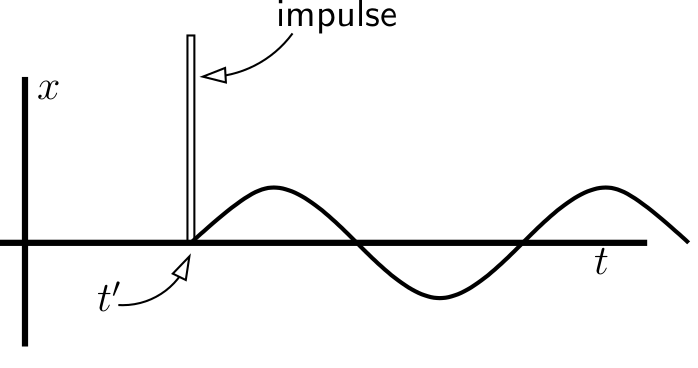
\includegraphics[width=0.44\textwidth]{figs/impulse.png}\\
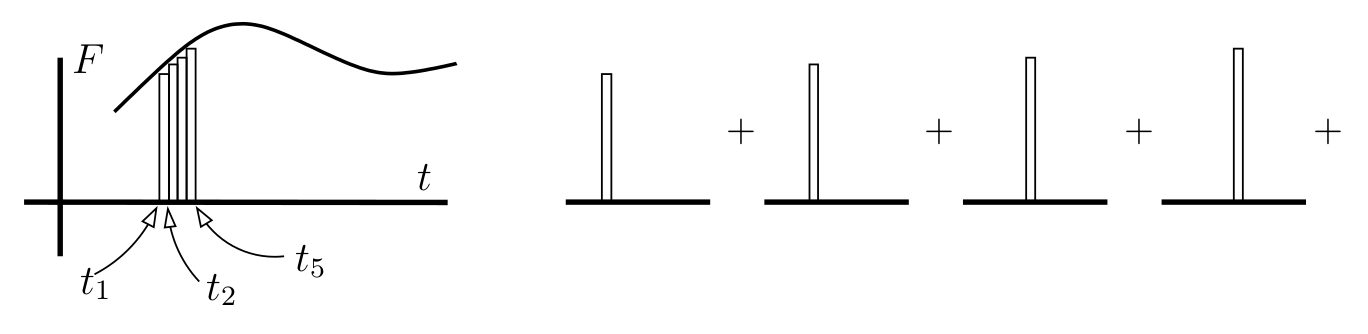
\includegraphics[width=0.90\textwidth]{figs/manyimpulses.png}
\caption{Top: The response of the variable $x$ to a delta function kick at 
$t'$. Bottom: A general force $f$ thought of as the sum of many impulses.
Figure taken from Quintin and Daniel's math methods notes.}
\label{fig:impulse}
\end{figure}

A possibility for $f$ is to use a Dirac delta function
$\delta(t-t')$; in physical contexts, this can be interpreted as a 
kick or {\it impulse}\index{impulse} delivered at time $t'$, and 
the resulting behavior for $x$ is the system's {\it response}\index{response} 
to the kick. This situation is depicted schematically in the top panel of
\figref{fig:impulse}. In such a case, the differential equation
\equatref{eq:diffyq} would become
\begin{equation}\label{eq:greenDelta}
  D_t\,x(t)=\delta(t-t').
\end{equation}
Let's give a special name to the solution of \equatref{eq:greenDelta}: We
are going to call it the {\it Green's function} $G(t-t')$, and it will
therefore satisfy
\begin{equation}\label{eq:greenDeltaSol}
  D_t\,G(t-t')=\delta(t-t').
\end{equation}
But now we are in a position to solve a wide class of differential equations
generally, by taking advantage of the fact that
\begin{equation}\label{eq:deltaSift}
  f(t)=\int\dd{t'}f(t')\delta(t-t').
\end{equation}
One way to interpret the above equation is that this force $f$ is being
constructed from a series of impulses, which is depicted schematically
in the bottom panel of \figref{fig:impulse}. Breaking down the force
in this way, the solution to our general equation \equatref{eq:diffyq} is
\begin{equation}\label{eq:greenSol}
  x(t)=\int\dd{t'}G(t-t')f(t').
\end{equation}
In other words, if we can solve \equatref{eq:greenDelta}, then we can
solve \equatref{eq:diffyq} by using \equatref{eq:greenSol}, almost
regardless of what $f$ is\footnote{I say ``almost" because $f$ must, for
example, be well-behaved enough that the delta function sifting works.}.
Equation~\eqref{eq:greenSol} takes the form of a convolution, and an
intuitive way to look at this convolution is
\begin{equation}
  \text{``output"} = \text{``system response to kicks"} * \text{``input"}.
\end{equation}

In the following two subsections, we are going to solve some
archetypal differential equations using Green's functions. These are
extremely relevant for QFT, and hopefully will help your intuition there.

\index{diffusion equation}
\subsection{The diffusion equation}

We start with a quick reminder about general diffusion equations.
The first core
principle underlying diffusion equations is a conservation law, i.e.
given some generic density $\rho$ depending on $\vec{x}$ and $t$,
\index{continuity equation}
one usually begins with a {\it continuity equation},
\begin{equation}\label{eq:continuityEquation}
  \pdv{\rho}{t}+\nabla\cdot\left(\rho\vec{v}\right)=0,
\end{equation}
where $\vec{v}$ is the velocity of the stuff at position $\vec{x}$. 
To interpret the continuity equation, one thinks about some finite region
in space $V$ and makes use of the divergence theorem to find
\begin{equation}
  \pdv{t}\int_V \dd[3]{x}\rho
     +\int_{S}\dd{\vec{S}}\cdot\left(\rho\vec{v}\right)=0.
\end{equation}
The integral in the first term on the LHS is just the total amount of
stuff enclosed in $V$, while the second term represents the amount of
stuff which is leaving $V$, passing through its surface $S$. In other
words, the continuity equation tells you that rate of change of stuff
in a volume equals the amount of stuff entering it--a formal statement
of an obvious\footnote{Actually while I called this fact obvious,
I guess it is not necessarily. For instance the discovery of mass conservation
is often credited to Antoine Lavoisier, who in the 1770s showed that 
the total mass of a burning system remains unchanged by weighing it
in closed vessels. Before this discovery, the prevailing ``phlogiston"
theory maintained that phlogiston, a conjectured fire-like element,
was released during combustion. Lavoisier was ultimately beheaded
during the French revolution~\cite{wiki:phlogiston,wiki:laviosier}.} fact. 

The second core principle is that when stuff diffuses, it flows from regions
of high concentration to regions of low concentration. This is
sometimes referred to as {\it Fick's law}\index{Fick's law}, and it
can be written as
\begin{equation}\label{eq:ficksLaw}
  \rho\vec{v}+D\nabla\rho=0,
\end{equation}
where $D$ is a constant called the {\it diffusion coefficient}. Combining
\equatref{eq:continuityEquation} and \eqref{eq:ficksLaw}, one finds
\begin{equation}
  \pdv{\rho}{t}-D\nabla^2\rho = 0.
\end{equation}
This is the {\it diffusion equation} in 3+1 dimensions. For the remainder
of this section, to keep the notation light, we will solve the diffusion
equation in 1+1 dimensions.

%\subsection{Perturbation theory}

\section{Dirac algebra}
In this section we summarize Section~3.2 of 
Ref.~\cite{peskin_introduction_1995}.
{\it Gamma matrices} appear when one works with spin-$1/2$ representations of
the Lorentz group. Here we remind the reader of algebraic properties of gamma
matrices. We work in 4D Minkowski space and demand that
\begin{equation}
  \left\{\gamma^\mu,\gamma^\nu\right\}=2g^{\mu\nu}\id,
\end{equation}
where $\id\equiv\id_4$. The representation of the Lorentz algebra is then
\begin{equation}
  S^{\mu\nu}=\frac{i}{4}\left[\gamma^\mu,\gamma^\nu\right].
\end{equation}
An explicit 4D representation of the gamma matrices, called the {\it chiral} 
\index{representation!chiral}\index{representation!Weyl}
or {\it Weyl} representation, uses the Pauli matrices:
\begin{equation}
  \gamma^0=\left(\begin{array}{cc}
                 0      & \id_2    \\
                 \id_2  & 0
           \end{array}\right), \qquad
  \gamma^i=\left(\begin{array}{cc}
                 0         & \sigma^i \\
                 -\sigma^i & 0
           \end{array}\right).
\end{equation}
In this representation, generators of boosts and rotations are, respectively,
\begin{equation}
  S^{0i}=\frac{i}{4}\left[\gamma^0,\gamma^i\right]
        =-\frac{i}{2}
         \left(\begin{array}{cc}
           \sigma^i & 0        \\
           0        & -\sigma^i
         \end{array}\right)
\end{equation}
and
\begin{equation}
  S^{ij}=\frac{i}{4}\left[\gamma^i,\gamma^j\right]
        =\frac{1}{2}\epsilon^{ijk}
         \left(\begin{array}{cc}
           \sigma^k & 0        \\
           0        & \sigma^k
         \end{array}\right).
\end{equation}
A four-component field that transforms under boosts and rotations according to
\index{spinor}
the above generators is called a {\it Dirac spinor}, which we usually denote
with $\psi$. 

Knowing a little bit about gamma matrices, we can introduce
``Feynman slash" notation,\index{slash notation}
\begin{equation}
  \slashed{p}\equiv\gamma_\mu p^\mu,
\end{equation}
and we can then write the {\it Dirac equation} in natural units as
\begin{equation}
  (i\slashed{\partial}-m\id)\psi=0.
\end{equation}
Next we define
\begin{equation}
  \bar{\psi}\equiv\psi^\dagger\gamma^0,
\end{equation}
which allows us to write down the Lorentz scalar $\bar{\psi}\psi$ and
the Lorentz vector $\bar{\psi}\gamma^\mu\psi$. The matrix
\begin{equation}
  \gamma_5=i\gamma^0\gamma^1\gamma^2\gamma^3
\end{equation}
allows us to define left-handed and right-handed projection operators
\begin{equation}\label{eq:projdef}
  P_L\equiv\frac{1}{2}(1-\gamma_5)~~~~\text{and}~~~~
  P_R\equiv\frac{1}{2}(1+\gamma_5),
\end{equation}
which project out the left-handed and right-handed components of Dirac spinors
like
\begin{equation}\label{eq:projact}
  \psi_R=P_R\psi,~~~~
  \psi_L=P_L\psi,~~~~
  \bar{\psi}_R=\bar{\psi}P_L,~~~~\text{and}~~~~
  \bar{\psi}_L=\bar{\psi}P_R.
\end{equation}
The following Propositions tell us how to manipulate gamma matrices and
projection operators.
\begin{proposition}{}{gammatech}
Gamma matrix identities in $4D$:
\begin{center}\begin{tabular}{lrcl}
1. &$\gamma_5^2$ &=& $\id$;\\
2. &$\left\{\gamma^\mu,\gamma_5\right\}$ &=& $\zd$;\\
3. &$\tr\left[\text{odd no. of $\gamma$s}\right]$ &=& $\zd$;\\
4. &$\slashed{a}\slashed{b}$ &=& $-\slashed{b}\slashed{a}-2(ab)\id$;\\
5. &$\tr\gamma^\mu\gamma^\nu$ &=& $-4g^{\mu\nu}\id$;\\
6. &$\gamma_\mu\gamma^\mu$&=& $-4\id$. 
\end{tabular}\end{center}
\end{proposition}
\begin{proposition}{}{projection}
Projection operator identities:
\begin{center}\begin{tabular}{lrcl}
1. & $P_R^2$ &=& $P_R$;\\
2. & $P_L^2$ &=& $P_L$;\\
3. & $\gamma^\mu P_L$ &=& $P_R \gamma^\mu$;\\
4. & $\gamma^\mu P_R$ &=& $P_L \gamma^\mu$.
\end{tabular}\end{center}
\end{proposition}

\bibliographystyle{unsrtnat}
\bibliography{bibliography}
